\chapter{A Conceptual Framework for Information Discovery and Curation on the Web}
\label{chapter:framework}

Although Web-based information discovery and curation tasks are commonly performed today, as we mentioned above, there is a lack of literature on how to support them when building applications. We reduce this gap by presenting a framework of design factors facilitating digital information discovery and curation (see Figure~\ref{fig:overview}). 

The framework consists of two main categories (discovery and curation) that are consequently decomposed into subcategories. Each subcategory contains factors that determine use case enablers and corresponding questions that can help application design and evaluation. Every component in the framework has corresponding automation and support techniques that improve user experience. This chapter outlines the main components of the framework. 


\begin{figure}[ht!]
	\noindent
	\centering
	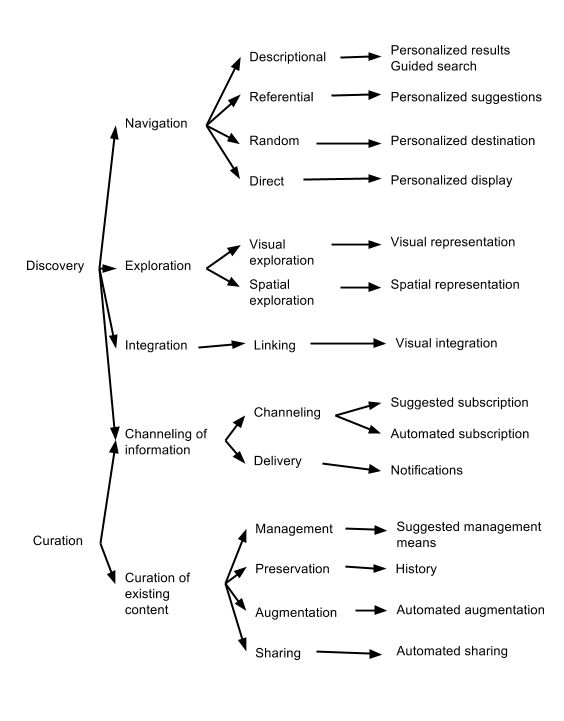
\includegraphics[width=\linewidth]{overview.png}
	\caption{Conceptual Framework Overview}
	\label{fig:overview} 
\end{figure}



{\section{Discovery and Navigation}
In order to discover information, a user needs to have a way of navigating to it. Common methods for navigation include descriptional navigation, referential, random, and direct. 


\begin{table}[ht!]
\caption{Mechanisms for Navigation}
\begin{tabular}{{|p{0.35\linewidth}|p{0.60\linewidth}|}}
\hline
Navigation mechanisms      & Questions to be posed during the design or evaluation of Web-based information discovery or curation tools \\
\hline
\textbf{Descriptional}     &                                                                                                            \\
Search-based navigation    & Does the search engine help retrieve diverse resources related to the topic of interest?                   \\
\textbf{Referential}       &                                                                                                            \\
Category-guided navigation & Do categories suggest and help with navigating to resources related to the topic of interest?              \\
Facet-guided navigation    & Do facets suggest and help with navigating to resources related to the topic of interest?                  \\
Filters-guided navigation  & Do filters suggest and help with navigating to resources related to the topic of interest?                 \\
Interest-guided navigation & Do interests suggest and help with navigating to resources related to the topic of interest?               \\
Tag-guided navigation      & Do tags suggest and help with navigating to resources related to the topic of interest?                    \\
Search by resource         & Can the user search by resource?                                                                           \\
\textbf{Random}            &                                                                                                            \\
Random navigation          & Is it possible to randomly skip through resources?                                                         \\
\textbf{Direct}            &                                                                                                            \\
Direct display             & Is any information displayed directly without search?      \\
\hline

\end{tabular}
\end{table}

\begin{table}[ht!]
\caption{Automation for Navigation}
\begin{tabular}{{|p{0.35\linewidth}|p{0.60\linewidth}|}}
\hline
Automation                   & Questions                                                     \\
\hline
\textbf{Descriptional}       &                                                               \\
Personalized results         & Does the descriptional mechanism return personalized results? \\
Guided search                & Is the descriptional mechanism guided?                        \\
\textbf{Referential}         &                                                               \\
Aggregating inerests         & Are interests aggregated?                                     \\
Suggesting similar resources & Does the application suggest similar resources?               \\
Suggesting tags              & Does the application suggest similar tags?                    \\
\textbf{Random}              &                                                               \\
Personalized destination     & Is random navigation personalized to the user?                \\
\textbf{Direct}              &                                                               \\
Tailoring display            &     Is direct display personalized to the user?   \\                                                       
\hline

\end{tabular}
\end{table}
} % end section

{\section{Exploration and Discovery}
\begin{table}[ht!]
\caption{Support for Exploration}
\begin{tabular}{{|p{0.35\linewidth}|p{0.60\linewidth}|}}
\hline

Method of exploration                       &          Questions                                                                             \\
\hline
\textbf{Visual exploration}                 &                                                                                       \\
Visual exploration of a single resource     & Does the system provide means for visual resource exploration?                        \\
Visual exploration of multiple resources    & Does the system provide means for visual resource exploration for multiple resources? \\
\textbf{Spatial exploration}                &                                                                                       \\
Spatial exploration of a single resource    & Does the system provide means for spatial resource exploration?                       \\
Spatial exploration of a multiple resources & Does the system provide means for spatial exploration for multiple resources?        \\                                                       
\hline

\end{tabular}
\end{table}

\begin{table}[ht!]
\caption{Support for Exploration of Multiple Resources}
\begin{tabular}{{|p{0.35\linewidth}|p{0.60\linewidth}|}}
\hline
Method of exploration of multiple resources & Questions                                    \\
\hline
\textbf{Visual exploration}                 &                                              \\
Visual preview                              & Are there visual previews of resources?      \\
Textual preview                             & Are there textual previews of resources?     \\
\textbf{Spatial exploration}                &                                              \\
List                                        & Are resources presented in a list?           \\
Grid                                        & Are resources presented in a list?           \\
Gallery                                     & Are resources presented in a gallery layout? \\
Consistent representation                   & Are resources presented in a consistent way?  \\                                                       
\hline

\end{tabular}
\end{table}

\begin{table}[ht!]
\caption{Support for Exploration of a Single Resource}
\begin{tabular}{{|p{0.35\linewidth}|p{0.60\linewidth}|}}
\hline
Method of exploration of single resource & Questions                                    \\
\hline
\textbf{Visual exploration}              &                                              \\
Visual cues                              & Are there visual cues?                       \\
Textual cues                             & Are there textual cues?                      \\
\textbf{Spatial exploration}             &                                              \\
Spatial semantic                         &                                              \\
Consistent representation                & Are resources presented in a consistent way?\\                                                       
\hline

\end{tabular}
\end{table}
} % end section
{\section{Integration}
\begin{table}[ht!]
\caption{Integration}
\begin{tabular}{{|p{0.35\linewidth}|p{0.60\linewidth}|}}
\hline
Integration mechanism  & Questions                                          \\
\hline
\textbf{Integration} &                                                    \\
Linking   & Is application linked to another application?\\                                                       
\hline

\end{tabular}
\end{table}

\begin{table}[ht!]
\caption{Support for Integration}
\begin{tabular}{{|p{0.35\linewidth}|p{0.60\linewidth}|}}
\hline
Integration support  & Questions                                          \\
\hline
\textbf{Integration} &                                                    \\
Visual integration   & Is another application's data visually integrated?\\                                                       
\hline

\end{tabular}
\end{table}
} % end section

{\section{Curation}

\begin{table}[ht!]
\caption{Curation Mechanisms}
\begin{tabular}{{|p{0.35\linewidth}|p{0.65\linewidth}|}}
\hline
Curation support  & Questions                                          \\
\hline
\textbf{Management}                   &                                                                                                           \\
List-based categorization               & Does the application support sorting information into list-like structures, either privately or publicly?                                                  \\
Tag-based categorization               & Does the application support tagging, either privately or publicly?                                                \\

\textbf{Preservation}                  &                                                                                                           \\
Internal preservation of internal resources       & Does the application support bookmarking mechanism(s) for preserving internal information within the application?        \\
Internal preservation of external resources       & Does the application support bookmarking mechanism(s) for preserving external information within the application?        \\
External preservation of internal resources      & Does the application support bookmarking mechanism(s) for preserving internal information outside of the application? \\ 

\textbf{Augmentation}            &                                                                                                           \\
Evaluation                   & Can the resource evaluations be recorded privately or publicly? \\
Annotation                   & Can resources be annotated privately or publicly?                                                                               \\    
       
\textbf{Sharing}           &                                                                                                           \\
Adding resources             & Can resources be publicly added to the collection of information within the application from other Web pages?     \\
Internal sharing         & Can internal resources be publicly reshared within the application?         \\ 
External sharing          & Can internal resources be publicly reshared outside of the application?         \\ 
\hline        
\end{tabular}
\end{table}

\begin{table}[ht!]
\caption{Curation Support}
\begin{tabular}{{|p{0.35\linewidth}|p{0.65\linewidth}|}}
\hline
Curation support  & Questions                                          \\
\hline
\textbf{Management}                   &                                                                                                           \\
Suggesting collections               & Does the application suggest relevant collections?                                                 \\
Suggesting tags               & Does the application suggests relevant tags?  \\

\textbf{Preservation}                  &                                                                                                           \\
History       & Does the application automatically preserve found information?        \\


\textbf{Augmentation}            &                                                                                                           \\
Automatic augmentation                   & Does the application automatically annotates resources? \\
 \\    
       
\textbf{Sharing}           &                                                                                                           \\
Automatic sharing& Are resources shared automatically? \\

\hline        
\end{tabular}
\end{table}

} % end section
{\section{Integration}
\begin{table}[ht!]
\caption{Integration}
\begin{tabular}{{|p{0.35\linewidth}|p{0.60\linewidth}|}}
\hline
Integration mechanism  & Questions                                          \\
\hline
\textbf{Integration} &                                                    \\
Linking   & Is application linked to another application?\\                                                       
\hline

\end{tabular}
\end{table}
} % end section

{\section{Chanelled Curation and Discovery}

\begin{table}[ht!]
\caption{Chenneling Mechanisms}
\begin{tabular}{{|p{0.35\linewidth}|p{0.60\linewidth}|}}
\hline
Channelling mechanisms     & Questions                                               \\
\hline
\textbf{Subscriptions}     &                                                         \\
User subscription          & Can the user subscribe to activities of other users?    \\
Site subscription          & Can the user subscribe to site updates?                 \\
Artifact subscription      & Can the user subscribe to artifact updates?             \\
\textbf{Notifications}     &                                                         \\
User activity overview     & Does the application display activities of other users? \\
Site activity overview     & Does the application display site updates?              \\
Artifact activity overview & Does the application display activities of other users?\\                                                       
\hline

\end{tabular}
\end{table}

\begin{table}[ht!]
\caption{Chenneling Support}
\begin{tabular}{{|p{0.35\linewidth}|p{0.60\linewidth}|}}
\hline
Channelling support               & Questions                                                          \\
\hline
\textbf{Subscriptions}            &                                                                    \\
Suggesting users                  & Are users suggested to the user?                                   \\
Automatic subscription            & Can the system subscribe the user automatically?                   \\
Suggesting artifacts              & Are artifacts suggested to the user?                               \\
\textbf{Notifications}            &                                                                    \\
User activity update notification & Does the application display activities of other users?            \\
Site activity update notification & Does the application notify the user about site updates?           \\
Artifact update notification      & Does the application notify the user about updates on an artifact?\\                                                       
\hline

\end{tabular}
\end{table}

} % end section

{\section{A Conceptual Framework for Information Discovery and Curation on the Web}
\begin{table*}[htbp]
\caption{Conceptual Framework}
\centering
\small
\begin{tabular}{|p{0.28\linewidth}|p{0.72\linewidth}|}
\hline
\textbf{\large{Design factors}}   & \textbf{\large{Questions to be posed during the design or evaluation of Web-based information discovery or curation tools 
}}  \\
\hline
&\\
\textbf{\large{Discovery}}                     &                                                                                                           \\

&\\
\emph{\textbf{Serendipitous discovery}}     &                                                                                                           \\

Arbitrary navigation         & Does the application provide a means for arbitrary navigation among resources?                              \\
Search-based navigation      & Does the search engine help retrieve diverse resources related to the topic of interest?               \\
Category-guided navigation & Do categories suggest and help with navigating to resources related to the topic of interest?           \\
Integration                  & If resources originate from a different site, do they link to their original sources?                   \\
Visual link preview               & If resources are delivered as links, do they have visual previews?                                                                        \\
Spatial arrangement          & Is there a semantic to the spatial arrangement of resources?                                                    \\
&\\
\emph{\textbf{Fact discovery}}                &                                                                                                           \\
Search-based navigation      & Does the search feature help discover the specific resource of interest?                                  \\
Category-guided navigation & Do categories help narrow results to specific types of resources?                                   \\
Integration                  & If resources originate from a different site, do they link to their original sources?                   \\
Uniform representation       & If resources are uniform, are they presented in a uniform way? \\
Visual link preview               & If resources are delivered as links, do they have visual previews?                                                                        \\
Spatial arrangement          & Is there a semantic to the spatial arrangement of resources?                                                    \\
&\\
\emph{\textbf{Rediscovery}}                     &                                                                                                           \\
History-based rediscovery    & Does the application save and provide access to browsing history?                                        \\
Bookmark-based rediscovery   & Does the application support bookmark-based resource revisitation?                                        \\
Search-based rediscovery     & Is the search a reliable method for resource revisitation?                             \\
&\\
\emph{\textbf{Channel-based discovery}}          &                                                                                                           \\
Site subscription            & Does the application allow subscriptions to news and updates?                                             \\
User subscription             & Does the application allow subscriptions to other users' activities?                                      \\
Notifications                & Does the application have one or more notification mechanisms?                                                      \\
Subscription to news feed                  & Can subscription updates be visible within the application?  \\
Content news feed                  & Can content updates be visible within the application? \\
&\\
\hline     
&\\                                        
\textbf{\large{Curation}}                     &                                                                                                        \\     
&\\  
\emph{\textbf{Management}}                    &                                                                                                           \\
List-based categorization               & Does the application support sorting information into list-like structures, either privately or publicly?                                                  \\
Tag-based categorization               & Does the application support tagging, either privately or publicly?                                                  \\
&\\
\emph{\textbf{Preservation}}                   &                                                                                                           \\
Internal preservation of internal resources       & Does the application support bookmarking mechanism(s) for preserving internal information within the application?        \\
Internal preservation of external resources       & Does the application support bookmarking mechanism(s) for preserving external information within the application?        \\
External preservation of internal resources      & Does the application support bookmarking mechanism(s) for preserving internal information outside of the application? \\ 
&\\
\emph{\textbf{Augmentation}}            &                                                                                                           \\
Evaluation                   & Can the resource evaluations be recorded privately or publicly? \\
Annotation                   & Can resources be annotated privately or publicly?                                                                               \\    
&\\        
\emph{\textbf{Sharing}}            &                                                                                                           \\
Adding resources             & Can resources be publicly added to the collection of information within the application from other Web pages?     \\
Internal sharing         & Can internal resources be publicly reshared within the application?         \\ 
External sharing          & Can internal resources be publicly reshared outside of the application?         \\ 
&\\           
\hline
\end{tabular}
\end{table*}



} % end section

{\subsection{Information Discovery}

\emph{RQ1: How do existing Web applications support information discovery?}

In our framework, we built on existing classifications of information seeking tasks and methods (see Sec. 2) and existing Web tools (see Table 1) to derive corresponding design factors. The discovery category consists of serendipitous discovery, fact discovery, rediscovery, and channel-based discovery. 
} % end subsection

{\subsubsection{Serendipitous Discovery}
Serendipitous discovery refers to information discovery resulting from serendipitous browsing. Such discovery is characterized by under-defined, absent, or hidden information needs, and it usually involves browsing through diverse resources with varying content types ~\cite{kellar2006, kellar2007}. Here, resource is defined as a collection of information about a single unit of inquiry, usually bundled together for presentation purposes. Some examples of resources are places, images, blog posts, and Web pages. The following are key criteria that influence serendipitous information discovery.

\textbf{Arbitrary navigation.} In order to browse diverse information, an information discovery tool needs to provide a way to arbitrarily navigate among resources, thereby supporting serendipitous information discovery ~\cite{foster}. Many applications, such as Tumblr and StumbleUpon, support arbitrary navigation to allow for opportunistic jumping from one resource to another. 

\textbf{Search-based navigation.} Search-based navigation often serves as an entry point for information seeking ~\cite{levene}. In case of serendipitous discovery, since the information need is not well articulated, the search engine should retrieve diverse resources related to a topic. For instance, searching for a location within Pinterest returns numerous images of the location that link to (or integrate with) other resources, blogs, and Web pages, whereas searching for the same place on Google Maps usually returns a small set of possible locations with limited information about those places.

\textbf{Category-guided navigation.} Similar to search-based navigation, category-guided navigation should provide a way to narrow the results to those related to one topic. In addition, categories can help the user formulate an information need by suggesting topics ~\cite{levene}. For example, when using Google Images, every search query suggests related categories of images to help users define an information need.

\textbf{Integration.} To users with ambiguous information needs, one information portal might not provide access to all information of interest. If an information discovery application gives access to resources from various sources, such as other Websites, the user should be able to navigate back to those sources.

\textbf{Visual link preview.} Abrams et al. ~\cite{abrams} identified link representation as one of the problems with traditional bookmarking. Analogous with browsing through a bookmark manager, identifying relevant information when browsing through links to diverse resources can be a challenging task. A visual preview should make it easier to evaluate the relevance of resources. Applications that facilitate serendipitous information discovery often employ elaborate resource representation techniques. Many social bookmarking systems, such as Scoop.it! and StumbleUpon, support visual previews of bookmarked pages. Delicious is a social bookmarking application that lacks this type of link representation support, which makes it harder to determine if the link will lead to a relevant resource.

\textbf{Spatial arrangement.} Similar to link representation, spatial visualization of numerous links is another problem that occurs when browsing through diverse content ~\cite{abrams}. Therefore, a semantic to the spatial arrangement of resources is of major importance. Information discovery applications that support serendipitous discovery often have a special way of spatially arranging resources to make it easier to browse through large amounts of information. For example, many tools use a 'pinboard' layout of resources similar to Pinterest.



} % end subsubsection

{\subsubsection{Fact Discovery}
Fact discovery refers to information discovery resulting from the search for a specific piece of information. It is characterized by a well-defined information need and is easier to perform within systems that provide access to homogeneous types of information ~\cite{kellar2006, lindley}. The main challenge for designing applications for fact discovery is to facilitate the finding of a specific piece of information, leaving little room for uncertainly in the search results. Below is a list of factors that influence fact discovery. 

\textbf{Search-based navigation.} With fact discovery, an information need is known ~\cite{kellar2006, kellar2007}. Therefore, the goal of search-based navigation for fact discovery is to directly navigate to the resource of interest, as opposed to retrieving diverse information (as in serendipitous discovery). Contrary to search-based navigation for serendipitous browsing, with fact discovery, the search engine returns a small set of results, among which only one is typically of interest to the user.

\textbf{Category-guided navigation.} Category-guided navigation is used to direct the user to relevant resources ~\cite{levene}. In the case of fact discovery, such navigation should narrow the results to a specific type of resource so that further fact discovery is bounded by that type. For example, TripAdvisor lets the user choose among flights, hotels, vacation rentals, restaurants, and destinations.

\textbf{Uniform representation.} Uniform representation is a method of displaying diverse resources in a common way, with each resource having the same set of components ~\cite{herrera}. Such a representation assures that each resource has the same set of facts associated with it, and therefore, the user can afford to have expectations about information that can be found when looking for a specific fact. For example, Yelp displays rating, price range, and address for all restaurants, so not only is it easy to find specific information, but the user can have expectations about the content of resources within the application. On the contrary, searching Tumblr for a restaurant will return a chaotic collection of information about the place. 

\textbf{Integration.} Similar to serendipitous discovery, if an information discovery application provides access to resources from other Websites, the user should be able to navigate to those sites as they may contain the facts of interest. Integration for fact finding is especially important when it gives an opportunity to display specific information about resources that otherwise would not be accessible. For example, Google Maps displays business ratings as a result of its integration with Google+.  

\textbf{Visual link preview.} If an application provides links to resources, a visual preview makes it easier to recognize the relevance of the resource ~\cite{abrams}. Applications that support fact discovery often use visual link preview, similar to applications that support serendipitous browsing. However, the motivation behind having a link preview for fact finding is to make it possible to identify if the resource is indeed what the user is looking for. For example, searching for an actor in IMDb will return a list of actors and their photographs, so that the user can pick the one they are interested in.

\textbf{Spatial arrangement.} Similar to serendipitous information discovery, spatial arrangement of resources is important ~\cite{abrams} as a poor semantic to the arrangement can make it difficult to visually navigate to the facts of interest.


} % end subsubsection

{\subsubsection{Rediscovery}
Rediscovery refers to information discovery resulting from revisiting previously discovered resources ~\cite{tauscher}. The following is a list of factors that enable rediscovery.

\textbf{History-based rediscovery.} A Web application needs to automatically record browsing history in order to enable history-based rediscovery ~\cite{tauscher}. History-based rediscovery appears to be the least common rediscovery mechanism, however, it can still be found in some Web applications, such as Google Maps.

\textbf{Bookmark-based rediscovery.} Bookmark-based revisitation is one of the most common ways of information rediscovery ~\cite{abrams}. The majority of Web browsers are equipped with bookmarking features. However, some modern Web applications, such as YouTube and Pinterest, provide integrated mechanisms for bookmarking and bookmark-based information rediscovery. 

\textbf{Search-based rediscovery.} Search-based rediscovery is not always a reliable way of refinding information ~\cite{cockburn}. In information portals that provide access to fairly ambiguous information and that have information regularly repopulated and updated, the search feature is usually designed around retrieving information related to some topic, but is not very specific. In order to revisit a resource, search must provide consistent results. In information discovery applications that provide access to specific information, such as Wikipedia and Rotten Tomatoes, search can usually lead directly to a specific resource. However, within Web applications such as We Heart It or Pinterest, search-based rediscovery is often unreliable.

} % end subsubsection

{\subsubsection{Channel-based Discovery}
Channel-based discovery can incorporate two different information seeking tasks, monitoring and awareness. It occurs when information is suggested to users based on the content that they are subscribed to. If users can actively look for updates, then an application affords monitoring ~\cite{morrison}. If users can receive notifications about updates, then an application facilitates awareness ~\cite{bates2002, bates1986}. Channel-based information discovery is usually enabled at sites that have regularly updated content, such as Pinterest and YouTube.                            


\textbf{Site subscription.} Subscriptions to updates from a site help users follow the news ~\cite{java}. In order to support subscription-based discovery, an application must provide a subscription mechanism. For example, Rotten Tomatoes allows subscriptions to newsletters; however, it does not allow subscriptions to movie critics, as a user-based subscription mechanism would allow. 

\textbf{User subscription.} In some applications, the content is updated and curated by users, and users can subscribe to other users. Similar to site subscriptions, user subscriptions are subscriptions to activity updates from individual users rather than all content updates, and help with networking and following users' activities ~\cite{millen}. Such subscriptions help to further filter new content delivered to the user. 

\textbf{Notifications.} Notification mechanisms enable user awareness about new content on the subscribed channel ~\cite{millen}. Different applications provide various notification mechanisms including messages within the application, informative emails, and smartphone notifications.

\textbf{Subscription news feeds.} Displaying a news feed within the application further promotes awareness and can serve as a monitoring mechanism. For such. 

\textbf{Content news feeds.} Similar to displaying a subscription news feed, displaying a content news feed promotes awareness and can serve as a monitoring mechanism.

Information discovery tools can have different implementations depending on the purpose of discovery. Using the information discovery factors in our framework (see Table 2), we described and evaluated currently existing tools. Similarly, the framework can be used for identifying gaps in information discovery support and developing new technologies (see Sec. 5).   \\

} % end subsubsection

{\subsection{Information Curation}
\emph{RQ2: How do existing information discovery applications support information curation?}\\

Information discovery applications vary from being completely socially curated and populated by users, to those that lack any curation mechanisms. 
By definition, digital information curation is the notion of managing, preserving, and adding value to collections of information ~\cite{beagrie, wittaker}. Thus, the curation category consists of information management, preservation, information enhancement, and sharing.  
} % end subsection

{\subsubsection{Management}
Information management is one of the key elements of information curation ~\cite{beagrie, wittaker}. Information categorization mechanisms are prevalent in applications that have a lot of information that is hard to categorize automatically or can mean something different for each user. In the context of Web information management, the following factors play a major role.

\textbf{List-based categorization.} Resource categorization helps establish relationships between various resources ~\cite{beagrie, wittaker}. Allowing people to sort information using custom categories can aid rediscovery, discovery in a socially curated space, as well as add more value to resources.

\textbf{Tag-based categorization.} Similar to list-based categorization, tagging aids rediscovery, adds value to resources, and aids discovery, especially in a socially curated space ~\cite{gruber}.  For example, Pinterest supports tag- and list-based categorizations, where lists are represented as 'pinboards'. Tumblr, on the other hand, only supports tag-based categorization. In addition, Pinterest allows for private information categorization.

} % end subsubsection

{\subsubsection{Information Preservation}
Information preservation is a common Web task that is usually performed with the intent of revisiting information ~\cite{abrams, wittaker}. However, in the case of opportunistic Web use, information gathering is sometimes performed with just the goal of collecting information rather than revisiting it in the future ~\cite{lindley}. Bookmarking is a traditional way of preserving information and many Web applications provide diverse bookmarking mechanisms. 

\textbf{Internal preservation of internal resources.} Internal preservation of internal resources means bookmarking resources to be reaccessed within the same application. Such bookmarking facilitates information curation within the system.

\textbf{Internal preservation of external resources.} Internal preservation of external resources signifies bookmarking other Web pages within an application. 
  
\textbf{External preservation of internal resources.} External preservation means bookmarking resources so that they become available through other bookmarking systems. An application must facilitate integration with other applications in order to enable external preservation ~\cite{abrams}.

On We Heart It, users can preserve \textit{internal  information} using \textit{internal collections} and they can add information from \textit{external} Websites. However, there are no integrated means for bookmarking \textit{internal content} using other bookmarking systems.  

} % end subsubsection

{\subsubsection{Augmentation}
One of the most important elements of digital curation is augmentation: adding value to information ~\cite{beagrie, wittaker}. It is often performed within social bookmarking systems. Many Web applications allow users to add value to the resources they curate. 

\textbf{Evaluation.} Evaluation methods can have various forms. They usually take place in socially curated information systems. However, evaluation can also contribute to personal reflection and information preservation. In addition, many applications allow users to evaluate resources by rating them or recording other forms of approval or disapproval. Some sites, such as Wikipedia, do not allow any evaluation. 

\textbf{Annotation.} Annotations are metadata attached to a resource, such as comments and descriptions. Annotations make it easier to search for and interpret information. 
} % end subsubsection

{\subsubsection{Sharing}
Sharing information is key to empowering social information curation ~\cite{beagrie}. Therefore, the main components that facilitate sharing are adding resources, and external and internal information sharing.

\textbf{Adding resources.} Adding resources not only facilitates global Web information curation, but it also scales the information available through the system, providing more opportunities for information discovery. Resources can be created by users themselves, taken from some other sources online, or both. For example, YouTube allows users to upload their own videos, whereas Pinterest permits adding images from other sites in addition to users' personal images. 

\textbf{External sharing.} Sharing resources through different media supports channel-based information discovery within the media channels. Information discovery applications commonly allow for sharing information on popular networking sites outside the application.

\textbf{Internal sharing.} Resharing resources within the system supports channel-based information discovery. 
} % end subsubsection

Information curation is a common activity within many information discovery applications. By asking questions about application design with regards to information curation as in Table 2 of the conceptual framework, designers can find ways to add value to information and enable information exploitation over time).

The following section describes possible use of the conceptual framework and gives a concrete example of its application.